\chapter{Continuidade Espacial}

Até os capítulos anteriores deste livro estávamos preocupados em realizar estatísticas diretamente com os dados. Inicialmente  propomos o conceito de continuidade espacial que define o limiar entre as técnicas de estatística e de geoestatística. Como descrito no capítulo um no tópico de krigagem, o modelo de covariâncias é que define o processo de estimativa.  Este capítulo apresenta uma breve revisão teórica sobre variografia e os conceitos relevantes para investigar o comportamento espacial do fenômeno geológico.  Toda a conceituação teórica envolvida neste capítulo será de relevância para o entendimento dos capítulos posteriores. 

\section{Definição de continuidade espacial e variografia}

A continuidade espacial define o comportamento médio da variável regionalizada para direções determinadas.  Ela é uma propriedade intrínseca do fenômeno estudado e caracteriza sua organização espacial. 

A variografia utiliza de funções estatísticas para reconhecer a continuidade espacial da variável aleatória. São formulações bi-pontuais que requerem a disposição espacial das amostras, conjugando sempre pares de valores para um dado espaçamento. A Figura \ref{Figura5} demonstra o posicionamento de amostras dentro de um domínio D e a diferença vetorial de espaçamento h. 

\begin{figure}[h]
	\centering
	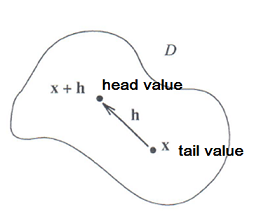
\includegraphics[scale=1.0]{Figura5}
	\caption{Notação geoestatística para a definição de um lag h em uma direção dentro de um domínio D de uma amostra com suporte x. Dois pares de pontos, um considerado head value, ou ponta do vetor e outro considerado tail value, ou início do vetor.}
	\label{Figura5}
\end{figure}

As funções de continuidade espacial medem comportamentos diferentes da variável aleatória: ou elas determinam a similaridade dos valores, ou determinam suas dissimilaridades . Essas propriedades são análogas às projeções vetoriais. A Figura \ref{Figura6} a demonstra a dissimilaridade como uma diferença de dois vetores, um vetor considerando os dados in situ e outro com os dados deslocados em um direção h. A diferença entre os vetores é analogamente comparada à função variograma em que são calculadas as médias das diferenças entre dados. Quanto maior for a discrepância entre os dados, maior será o vetor da diferença entre as amostras. A Figura \ref{Figura6} b também demonstra a similaridade dos dados como uma projeção vetorial, em que um conjunto mais similar apresenta maiores projeções. Nesse caso a similaridade analogamente comparada com o covariograma pode ser comparada com uma projeção de um vetor sobre outro ou com o produto escalar entre o vetor Z(x+h) e o vetor Z(x).

\begin{figure}[!]
	\centering
	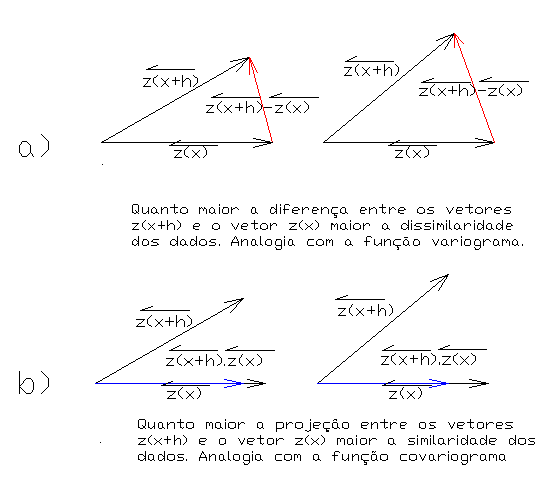
\includegraphics[scale=1.0]{Figura6}
	\caption{Funções de continuidade espacial como uma interpretação de vetores. a) Variograma como uma diferença de vetores b) Covariograma como uma projeção de vetores.}
	\label{Figura6}
\end{figure}

\section{Dependência espacial}

Para os fenômenos geológicos, é de se esperar que as amostras mais próximas apresentem maior similaridade de valores amostrados. A Figura \ref{Figura7} é uma representação gráfica desta característica comentada em um gráfico h-scatter para valores de lag crescentes. Quanto maior for a distância entre as amostras, mais estes pares de valores são dissimilares ou descorrelacionados.  

\begin{figure}[!]
	\centering
	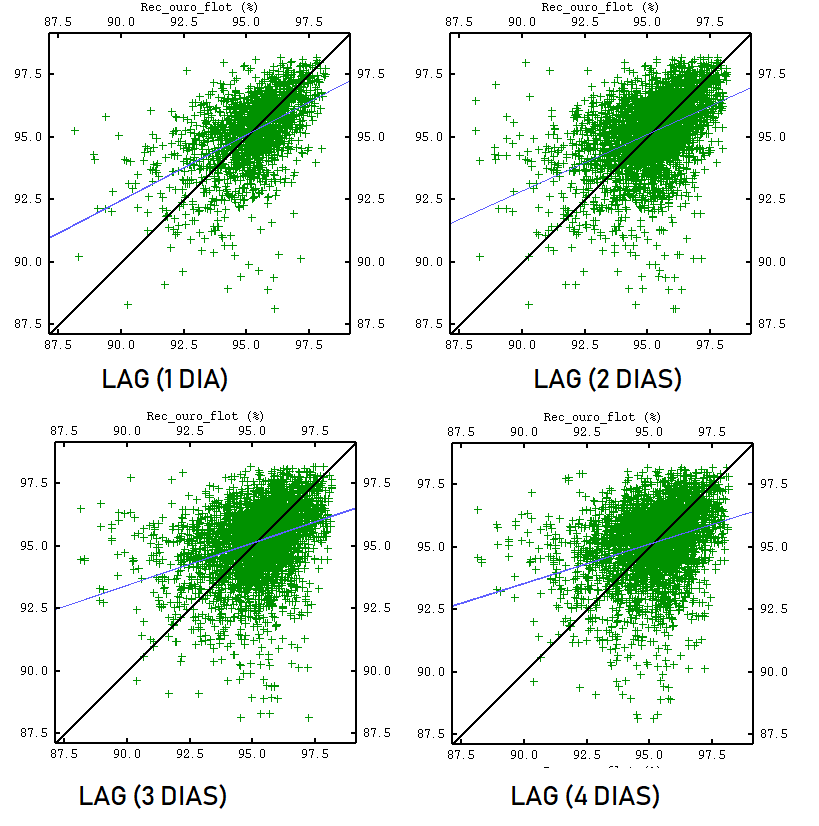
\includegraphics[scale=0.8]{Figura7}
	\caption{H-scatterplots de uma variável para lags de 0,1m , 0,2m, 0,3m e 0,4m. Aumento da descorrelação de acordo com o aumento do comprimento dos lags.}
	\label{Figura7}
\end{figure}

\section{Hipótese de estacionaridade}

As funções de continuidade espacial requerem que o modelo ajustado não seja afetado pela translação. A hipótese estacionaridade também pode ser denominada de invariância de translação. Alguns tipos de funções exigem hipóteses mais fortes, tal como a de estacionaridade segunda ordem. Esta admite que todas as distribuições das variáveis aleatórias no espaço possuam médias e variância iguais. 
Um exemplo da necessidade da estacionaridade de segunda ordem é a portabilidade das funções variograma e covariograma. As funções variograma e covariograma podem estão relacionadas quando estabelecido um regime estacionário de segunda ordem, resultando na Equação \ref{Equacao3}:

\begin{equation}\label{Equacao3}
\gamma(h) = C(0) - C(h)
\end{equation}

Em que $\gamma(h)$ é o semi-variograma, $C(0)$ é a variância à priori dos dados e $C(h)$ o valor do covariograma.  No entanto, a presença de tendência nos dados mostra que o covariograma e o variograma não se convertem em uma relação direta, pois a média da variável aleatória não é constante no domínio e por isso não implica em uma hipótese de estacionaridade de segunda ordem. 

\section{Funções experimentais de continuidade espacial}

\subsection{Efeito dos dados sobre os valores experimentais}

As funções clássicas de continuidade espacial são afetadas por valores extremos, esparcidade dos dados e valores clusterizados o que levou à investigação de funções de estimativas robustas. Leva-se em consideração que a continuidade espacial é uma propriedade do domínio e não das amostras. No entanto, pela escassez de informação, ela é inferida a partir de uma quantidade limitada de dados. Se as observações não cobrirem as dimensões do objeto de estudo, devido a um número pequeno de amostras com dados esparsos ou agrupados, a estimativa pode não representar a continuidade do fenômeno. Pode-se demonstrar a conexão entre o variograma experimental e a amostragem, tal que as amostras devem respeitar as seguintes definições:

\begin{enumerate}
	\item As amostras devem estar contidas na mineralização do depósito.
	\item Os corpos de minério devem ser tratados de forma diferenciada.
	\item Todas as amostras devem ter o mesmo suporte.	
\end{enumerate}

Um número crescente de amostragens pode nem sempre resultar em um benefício da informação sobre a continuidade espacial. Como as funções de continuidade espacial são valores médios de uma gama de pares de amostras no espaço, e os valores médios tendem a suavizar o efeito das informações, o acréscimo de pares de informações redundantes pode não alterar as funções de continuidade espacial. O reconhecimento da continuidade exige uma estratégia de amostragem adequada e depende complexidade do depósito mineral. Corpos com baixa continuidade espacial podem ser analisados com malhas adensadas em contrapartida de depósitos com alta continuidade espacial que podem ser analisados com malhas menos adensadas. 

\subsection{Funções de continuidade espacial mais comuns}

Matheron o criador da geoestatística desenvolveu as principais funções de estimativa da continuidade espacial para entender o comportamento das variáveis aleatórias regionalizadas. Duas destas são consideradas as mais tradicionais definidas inicialmente pelo autor. O covariograma e o variograma medem respectivamente a similaridade e dissimilaridade dos dados. Define-se a função covariograma pela Equação \ref{Equacao4}:

\begin{equation}\label{Equacao4}
C(h) = E\left[ \left( Z_{i+h} - m_{i+h} \right) \left( Z_i -m_i\right) \right] 
\end{equation}

Em que $Z_i$ é o valor da variável aleatória no suporte i, $Z_{i+h}$ é o valor da variável aleatória transladada por um vetor h e $m_{i+h}$ o valor médio da variável transladada. Sob a hipótese de estacionaridade de segunda ordem os valores da média são constantes tal que $m_{i+h}=m_i$ e a Equação \ref{Equacao4}  pode ser traduzida pela Equação \ref{Equacao5} por uma transformação algébrica: 

\begin{equation}\label{Equacao5}
C(h) = E\left( Z_{i+h}Z_i\right)  -m^2
\end{equation}

A função variograma pode ser representada pela Equação \ref{Equacao6}:

\begin{equation}\label{Equacao6}
2\gamma(h) = E\left[ \left( Z_{i+h}-Z_i\right)^2\right] 
\end{equation}

Em que $\gamma(h)$ é também denominado de semi variograma. Na literatura, é comum a utilização ambígua dos termos, referindo-se ao valor de semi variograma como a função variograma. A função semi variograma pode ser representada como uma distância da dispersão de pontos em relação à reta Y=X, em um gráfico h-scatterplot.  A Figura \ref{Figura8} é uma demonstração gráfica da interpretação do semivariograma como um valor médio das distâncias das variáveis Zu e Zu+h, com esses valores em x e y e com a reta de correlação máxima. A demonstração da Figura \ref{Figura8} em termos matemáticos está descrito na Equação \ref{Equacao7}:

\begin{figure}[h]
	\centering
	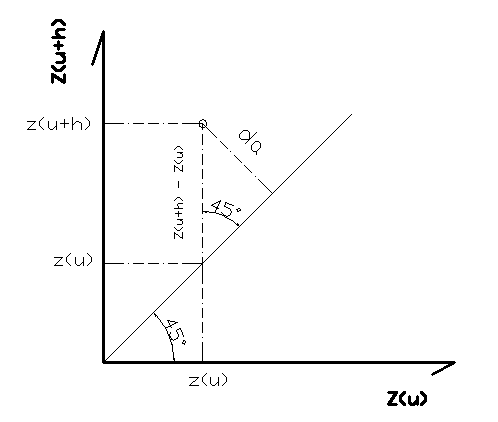
\includegraphics[scale=0.8]{Figura8}
	\caption{Interpretação geométrica do semi-variograma como sendo a distância de um ponto em relação a reta x=y.}
	\label{Figura8}
\end{figure}

\begin{equation}\label{Equacao7}
\frac{1}{n} \sum_{i=1}^{n} da^2 =\frac{1}{n} \sum_{i=1}^{n} sen^2(45^\circ)\left( z_i -z_{i+h} \right)^2 = \frac{1}{2n} \sum_{i=1}^{n} \left( z_i -z_{i+h} \right)^2
\end{equation}

\subsection{Outras funções experimentais}

Várias são as funções de continuidade espacial utilizadas na bibliografia, principalmente as mais clássicas desenvolvidas por Matheron. No entanto, a busca de estimativas cada vez menos sensíveis aos valores extremos levou ao desenvolvimento de modelos robustos. Entre eles podemos citar o variograma relativo e o pairwise. Há também uma classe de diferentes tipos de estimativas para a função variograma, utilizando uma série de médias com limites aparados e dentre elas a própria mediana para poucos valores de pares. 

Modelos mais robustos de variograma estão desenvolvidos ao longo da bibliografia. A Equação \ref{Equacao8} demonstra a relação determinada pelos autores, que garante menores efeitos de valores extremos ao contrário do variograma tradicional proposto por Matheron, também denominada de Rodograma: 

\begin{equation}\label{Equacao8}
\gamma(h) = \frac{1}{2n} \sum_{i=1}^{n} \left|  Z_i - Z_{i+h} \right| ^\frac{1}{2}
\end{equation}

A Tabela \ref{Tabela 3} é uma representação das principais estimativas de funções de continuidade espacial. Alguns tipos tem maior recorrência que as demais como o variograma tradicional e a covariância, propostos inicialmente por Matheron:

Em que $m_i$ e $m_{i+h}$ são os valores médios determinados no início e na ponta do vetor ($E(Z_i)$ e $E(Z_{i+h})$) e  $\sigma_i^2$ e $\sigma_{i+h}^2$ são as variâncias no início e na ponta do vetor. No caso de estacionaridade de segunda ordem $m_i = m_{i+h}$ e  $\sigma_i^2 = \sigma_{i+h}^2$, no entanto as funções experimentais calculam à priori estes valores de acordo com as distribuições amostrais do tail e do head para cada diferença de lag. A obtenção dos valores experimentais das funções de continuidade espacial é a etapa inicial, que é seguida pela modelagem variográfica e pelas etapas posteriores de estimativa e simulações.

\begin{table}[h]
	\centering
	\caption{Funções de continuidade espaciais experimentais}
	\label{Tabela 3}
	\begin{tabular}{cc}
		\toprule
		\textbf{Função experimental} &  \textbf{Equação} \\\midrule \\
		Semi-variograma                      & $\sum_{i=0}^{n}\frac{\left( Z_i - Z_{i+h} \right)^2 }{2n} $      \\ \\
		Covariograma                        & $\frac{1}{n}\sum_{i=0}^{n} (Z_i-m_i).(Z_{i+h}-m_{i+h})$       \\ \\
		Correlograma                       & $\frac{1}{n}\sum_{i=0}^{n}\frac{ (Z_i-m_i).(Z_{i+h}-m_{i+h})}{\sigma_i\sigma_{i+h}}$   \\   \\
		Pair-Wise                       & $\frac{1}{n}\sum_{i=0}^{n} \frac{(Z_i-Z_{i+h})^2}{\left( \frac{Z_i + Z_{i+h}}{2}\right)^2}$      \\ \\
		Madograma                      & $\frac{1}{n} \sum_{i=0}^{n} \left| Z_i -Z_{i+h} \right|  $       \\ \\ 
		Variograma Relativo              & 
		$\frac{1}{n}\sum_{i=0}^{n} \frac{(Z_i-Z_{i+h})^2}{\left( \frac{m_i + m_{i+h}}{2}\right)^2}$      \\ \\ \bottomrule     
	\end{tabular}
\end{table}

O cálculo dos valores experimentais é realizado segundo uma direção vetorial. A Figura \ref{Figura9} demonstra os valores de amostras aceitáveis como pares de pontos permissíveis. Para um lag unitário, somente os valores adjacentes no grid estão disponíveis. A direção escolhida para o cálculo do variograma experimental é leste-oeste. 

\begin{figure}[!]
	\centering
	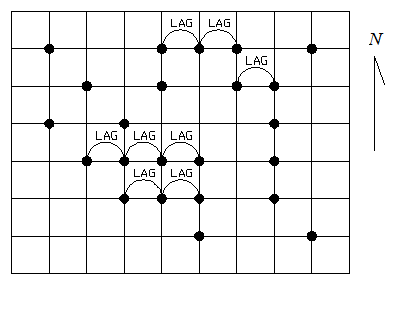
\includegraphics[scale=0.9]{Figura9}
	\caption{Cálculo de variogramas experimentais segundo um lag unitário na direção Leste-Oeste.}
	\label{Figura9}
\end{figure}

O mesmo pode ser representado na Figura \ref{Figura10}, em que os valores disponíveis como pares para o cálculo são efetuados em dois nós do grid consecutivos. 

\begin{figure}[!]
	\centering
	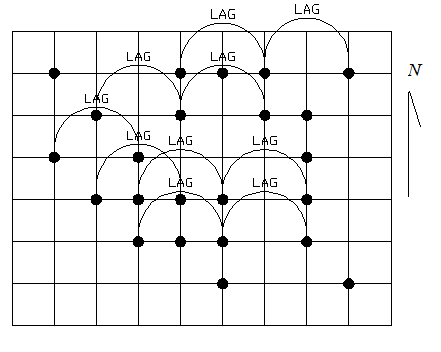
\includegraphics[scale=0.9]{Figura10}
	\caption{Cálculo de variogramas experimentais segundo o dobro do lag na direção leste-oeste.}
	\label{Figura10}
\end{figure}

Os valores calculados do variograma nas  Figuras \ref{Figura9} e \ref{Figura10} estão demonstrados em um gráfico na Figura \ref{Figura11} de forma ilustrativa como dois pontos consecutivos, P1 e P2 ligados por um modelo hipotético como forma ilustrativa. Cada diferença de lag representará um valor de variograma associado. 

\begin{figure}[!]
	\centering
	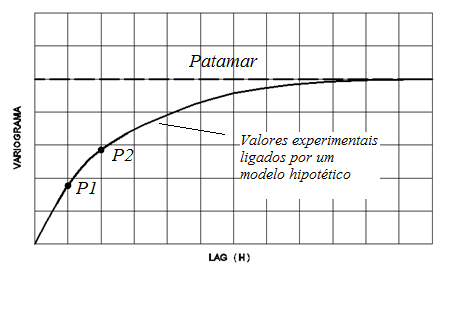
\includegraphics[scale=1.0]{Figura11}
	\caption{Função variograma experimental para os cálculos nas Figuras 9 e 10 e ajuste em um modelo hipotético. P1 e P2 representam os pontos para um lag unitário e o dobro do lag.}
	\label{Figura11}
\end{figure}

\subsection{Parâmetros de busca}

Nas Figuras \ref{Figura9} e \ref{Figura10}, a direção escolhida para o cálculo da função variograma permite medidas regulares. No entanto, a maioria dos casos relacionados à mineração é caracterizada por disposições irregulares das amostras. Neste caso, o variograma direcional não é mais calculado em uma direção absoluta, mas apresenta uma região de incerteza no alinhamento das amostras. A Figura \ref{Figura12} é uma representação da busca de pares irregularmente espaçados.

Para o problema bidimensional, são consideradas 3 variáveis geométricas de incerteza e o lag do vetor propriamente dito. As geometrias variáveis são:

\begin{enumerate}
	\item 	Tolerância angular = Desvio angular da direção nos lags de menor tamanho.
	\item 	Banda = Desvio lateral da busca. 
	\item	Tolerância linear = Desvio longitudinal da busca.
	
\end{enumerate}

\begin{figure}[!]
	\centering
	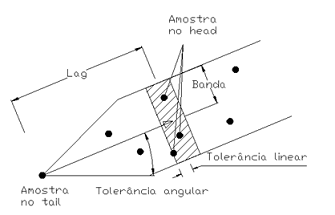
\includegraphics[scale=1.0]{Figura12}
	\caption{Busca de pontos da função de continuidade para amostras irregularmente espaçadas.}
	\label{Figura12}
\end{figure}

No caso tridimensional, a busca de pares pode se realizar de duas formas diferentes, sob uma perspectiva elíptica ou prismática. A Figura \ref{Figura13} é uma representação da busca de pares nas duas formas geométricas. 


\begin{figure}[!]
	\centering
	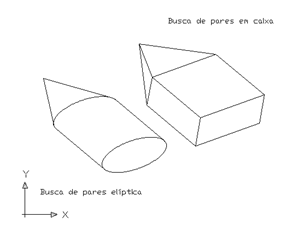
\includegraphics[scale=1.5]{Figura13}
	\caption{Busca de pares de pontos em uma direção tridimensional. Busca de pares elíptica utilizada no SGeMS e em caixa utilizada no GSLib.}
	\label{Figura13}
\end{figure}

A procura pela metodologia em caixa é utilizada no software Gslib, em que são estipuladas não somente a tolerância horizontal e a banda horizontal, como também a tolerância vertical e a banda vertical. A alternativa de caixa é preferencial à busca de pontos cilíndrica, pois em casos onde depósitos minerais apresentem estratigrafia característica, as bandas verticais e horizontais podem ser utilizadas para delimitação de amostras pertencentes ao mesmo nível de formação geológica. 

\section{Modelagem de funções de continuidade espacial}

\subsection{Modelos de variogramas permissíveis}

Após a estimativa dos valores experimentais, a análise variográfica procede com a modelagem de funções permissíveis e estabelecimento de um modelo simplificado de regionalização. Um modelo permissível de variograma deve possuir as seguintes características: 

\begin{enumerate}
	\item 	O modelo  deve ser uma função par $\gamma(h)= \gamma(-h)$.
	\item O modelo deve ser uma função positiva definida tal que qualquer combinação linear dos seus valores deve ser maior ou igual a zero, como demonstrado na Equação \ref{Equacao9}.
	\begin{equation}\label{Equacao9}
	\sum_{i=0}^{n}\sum_{j=0}^{n}\lambda_i\lambda_j\gamma(x_i-x_j) \geq 0
	\end{equation}
	Em que $\lambda_i$ é uma constante de proporcionalidade e $x_i$ e $x_j$ são as diferenças das amostras em um suporte i e j qualquer.
	\item Modelo deve ser limitado por um valor limite, geralmente caracterizado como a variância à priori do fenômeno.
	
\end{enumerate}

\subsection{Parâmetros das funções de continuidade}

O conjunto de variogramas transitivos, ou seja, que apresentam um patamar possuem parâmetros característicos. A Figura \ref{Figura14} é uma representação de um modelo de variograma. Os parâmetros da função são:

\begin{enumerate}
	\item	Efeito pepita: Caracteriza a dispersão dos valores para um lag imediatamente maior que zero. O Efeito pepita representa, além da variabilidade de escala, os erros associados à amostragem.
	
	\item 	Range ou alcance: Máxima distância de influência da correlação. A partir do range não mais existe correlação entre os pares de valores da variável aleatória e estes podem ser ditos independentes.
	
	\item Patamar: O patamar representa o estabelecimento da máxima dispersão admissível. Nas funções em que a similaridade é a propriedade caracterizada, o patamar assume valor nulo tal como na Figura \ref{Figura15}. A melhor estimativa para o patamar pode não ser a variância das amostras, mas deve-se considerar o posicionamento espacial destas pela utilização da variância de dispersão, da declusterização dos pesos, além do tratamento de valores extremos.
	
\end{enumerate}

\begin{figure}[!]
	\centering
	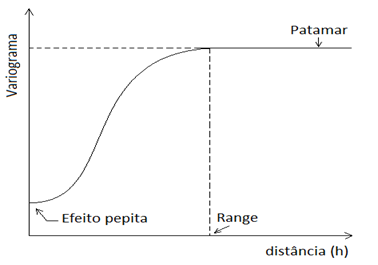
\includegraphics[scale=1.0]{Figura14}
	\caption{Parâmetros do variograma.}
	\label{Figura14}
\end{figure}

\begin{figure}[!]
	\centering
	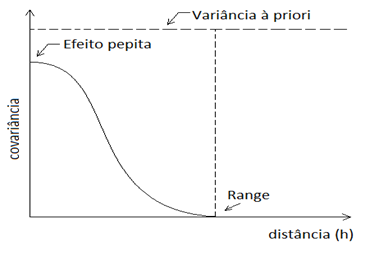
\includegraphics[scale=1.0]{Figura15}
	\caption{Parâmetros da função covariograma.}
	\label{Figura15}
\end{figure}

\subsection{Modelos de continuidade espacial mais comuns}

Dentre os modelos de covariância mais comuns podemos citar: 

Efeito de pepita puro: Considera o efeito de dispersão puro. Não representa nenhuma conectividade dos dados e a probabilidade de ocorrência de um determinado valor é caracterizada por uma distribuição uniforme. O efeito pepita pode ser caracterizado como uma percepção não linear do fenômeno em uma escala considerada. A Equação \ref{Equacao9_5} demonstra o modelo de variograma com efeito de pepita puro.

\begin{equation}\label{Equacao9_5}
\gamma(h) = \begin{cases}
0 & , h =0 \\
1 &,\text{ao contrário}
\end{cases}
\end{equation}


Modelo exponencial: O modelo representa o valor de variabilidade com decaimento exponencial. Apresenta-se assíntota no patamar e o range é caracterizado por um valor prático que ocupa 95\% da variância a priori quando h = 3a, sendo “a” o alcance prático. A Equação \ref{Equacao10} demonstra o modelo de variograma exponencial.

\begin{equation}\label{Equacao10}
\gamma(h) = 1 - \exp^{\frac{-h}{a}}
\end{equation}

Modelo Gaussiano: O modelo representa o valor de variabilidade de decrescimento exponencial quadrático. Dentre as funções, é a que apresenta maior suavização próxima da origem. Apresenta também um range prático tal que $h=a\sqrt{3}$. A Equação \ref{Equacao11} demonstra o modelo de variograma gaussiano.

\begin{equation}\label{Equacao11}
\gamma(h) = 1 - \exp^{-\frac{h^2}{a^2}}
\end{equation}

Modelo Esférico: A Equação \ref{Equacao12} é a representação de um modelo esférico. Apesar de constituir uma função de terceira ordem, que feriria os princípios de positiva definida, o modelo esférico é limitado pelo alcance da função, e a partir daquele valor é substituído pelo patamar. 

\begin{equation}\label{Equacao12}
\gamma(h) = \begin{cases}
\left( \frac{3h}{2a} - \frac{h^3}{2a^3} \right)  &, h < a \\
1 & , h >= a
\end{cases}
\end{equation}

Como todos os modelos prescritos são permissíveis então qualquer combinação destes também resulta em um modelo permissível. 

\subsection{Anisotropia}

A anisotropia é a mudança de comportamento das propriedades do variograma por rotação. Os fenômenos geológicos podem permitir a gênese diferenciada dos litotipos à partir de controles e enriquecimentos em sentidos distintos. Dois casos são recorrentes na literatura e envolvem a forma geométrica e zonal. 

O caso geométrico delimita alcances diferentes para um mesmo patamar. A anisotropia geométrica pode ser resumida em um modelo de elipsóide em que haverá eixos de máximo, médio e mínimo alcance. A Figura \ref{Figura16} é uma representação da anisotropia geométrica.

\begin{figure}[!]
	\centering
	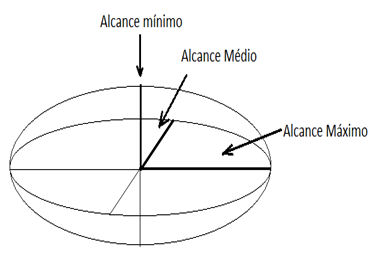
\includegraphics[scale=1.0]{Figura16}
	\caption{Representação do modelo de anisotropia geométrico. Elipsóide com valores de alcance mínimo médio e alcance máximo.}
	\label{Figura16}
\end{figure}

Os alcances em qualquer direção podem ser derivados de um modelo isotrópico unitário a partir de operações lineares, resultando em um novo sistema de coordenadas. A Equação \ref{Equacao13} representa a matriz de rotação das coordenadas para os eixos de referência.

\begin{equation}\label{Equacao13}
Q=\begin{bmatrix}
cos\theta_3 & sin\theta_3 & 0 \\
-sin\theta_3 & cos\theta_3 & 0\\
0 &0 & 1
\end{bmatrix}\begin{bmatrix}
1 & 0 & 0 \\
cos\theta_2 & sin\theta_2 & 0\\
-sin\theta_2 &cos\theta_2 & 0
\end{bmatrix}\begin{bmatrix}
cos\theta_1 & sin\theta_1 & 0 \\
-sin\theta_1 & cos\theta_1 & 0\\
0 &0 & 1
\end{bmatrix}
\end{equation}

Em que $\theta_3$ consiste no ângulo de rotação no eixo z, $\theta_2$ o ângulo de rotação no eixo y e $\theta_1$ a rotação do ângulo no eixo x.  Os valores do vetor unitário são então redimensionados segundo a matriz de dilatação da Equação \ref{Equacao14}.

\begin{equation}\label{Equacao14}
D=\begin{bmatrix}
l_1 & 0 & 0 \\
0 & l_2 & 0\\
0 &0 & l_3
\end{bmatrix}
\end{equation}

Em que $l_1$, $l_2$ e $l_3$ são os comprimentos dos eixos de máximo, médio e mínimo alcance. Tais matrizes são utilizadas para se construir o modelo do elipsoide de anisotropia e determinar os alcances em qualquer direção possível.

O caso zonal consiste em variações de patamares ao longo de direções diferentes. Demonstra-se o exemplo da anisotropia zonal. Observa-se na Figura \ref{Figura17} que a diferença de azimute pelo ângulo $\theta$ leva a uma diferença de patamares de g1 para g1 + g2. A anisotropia zonal é característica em alguns tipos de depósitos divididos em estratos, ao qual se verifica diferenças litológicas nas diversas camadas. A variabilidade na direção perpendicular aos estratos tende a ser diferente da direção paralela, que tende a ser mais contínua pelo princípio de sedimentação. 

\begin{figure}[!]
	\centering
	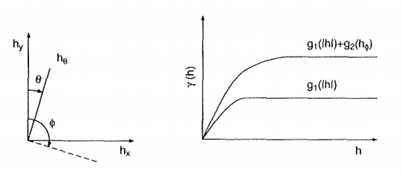
\includegraphics[scale=1.0]{Figura17}
	\caption{Anisotropia zonal representada nos variogramas a) Diferença entre as direções dos variogramas b) Representação da anisotropia por variogramas com patamares diferentes.}
	\label{Figura17}
\end{figure}

A modelagem de anisotropias zonais envolve a utilização de estruturas distintas de variograma que combinadas representarão o conjunto total. A anisotropia zonal também pode ser caracterizada como uma mudança de fenômeno em larga escala. 

A anisotropia é uma flexibilização do modelo de variograma para atender às necessidades de depósitos mais complexos, que podem apresentar características diferenciadas segundo diversas direções.

\subsection{Funções de continuidade espacial cruzadas}

Na modelagem espacial de múltiplas variáveis, tal como os modelos de cokrigagem ou markovianos, é necessário determinar funções de continuidade cruzadas além das diretas. Estas não estão submetidas às mesmas condições de contorno das funções diretas. Primeiramente, porque o valor de patamar de uma estatística cruzada é sempre menor ou igual a das estatísticas diretas e está ligado à correlação entre as variáveis utilizadas para a modelagem.  

O covariograma cruzado pode ser representada pela Equação \ref{Equacao15} em que Zi e Zj são variáveis distintas e mi e mj são suas respectivas médias: 

\begin{equation}\label{Equacao15}
C_{ij}(h) = \frac{1}{2} E\left[ \left( Z_i(x+h) -m_i \right) \left( Z_j(x) -m_j \right)\right] 
\end{equation}

O covariograma direto é uma função par e unicamente limitada por um valor de patamar. As funções cruzadas, no entanto, podem apresentar efeitos de retardo e não se comportarem como uma função par, tal que $C_{ij} (h)\neq C_{ij} (-h)$, e que i e j são variáveis aleatórias diferentes entre si. 
Toda função pode ser descrita como uma combinação de funções pares e ímpares. A covariância cruzada pode ser decomposta tal como na Equação \ref{Equacao16}:

\begin{equation}\label{Equacao16}
C_{ij}(h) = \frac{1}{2}\left( C_{ij}(h)+C_{ij}(-h)\right) +\frac{1}{2}\left( C_{ij}(h)-C_{ij}(-h)\right)
\end{equation}

Em que a soma de covariâncias representa o termo par da função e a diferença o termo ímpar. Há um sério problema em se definir a matriz de covariâncias, pois geralmente para um dado lag ela não poderá ser considerada nem positiva definida ou negativa definida. 

Os efeitos produzidos pelo retardo não permitem a utilização de funções assimétricas na resolução dos sistemas de krigagem utilizados a posteriori. Segundo o mesmo autor, a dificuldade de caracterização da covariância no espaço de valores reais leva a utilização em números complexos. 

O variograma cruzado, no entanto, não está sujeito aos efeitos do retardo tal como a covariância e apresenta unicamente um termo par. A Equação \ref{Equacao17} expressa a fórmula da função: 

\begin{equation}\label{Equacao17}
\gamma_{ij}(h) = \frac{1}{2}E\left[ \left( Z_i(x+h) - Z_i(x)\right) \left( Z_j(x+h) - Z_j(x)\right) \right] 
\end{equation}

\subsection{Modelo linear de corregionalização}

Segundo , o modelo linear de corregionalização implica que uma variável aleatória deve ser escrita como uma combinação linear de funções aleatórias independentes. Isso significa que para qualquer variável i e j, o modelo estrutural deve ser o mesmo, tal que $C(h)=\sum_{i=1}^{n} b_i\rho(h) $ e que $\rho(h)$ é um modelo único de correlograma e $b_i$ é a contribuição para cada variável considerada. Para ser considerado um modelo permissível, o traço da matriz de covariância deve ser maior que a soma de qualquer coluna ou linha, ou que o determinante deva ser maior ou igual a zero. Os modelos lineares de corregionalização devem satisfazer a condição de matrizes positiva definidas para a resolução dos casos multivariados. A dificuldade de se estabelecerem modelos segundo os critérios necessários, levou à simplificações das krigagens colocadas e de modelos Markovianos. 

\subsection{Modelagem automática de variogramas}

Na tentativa de minimizar o trabalho do avaliador na modelagem de funções cada vez mais complexas, a modelagem semiautomática também é uma alternativa para reduzir o erro do ajuste do modelo. Em 1985, já havia se iniciado a tentativa de modelagens automáticas por meio de mínimos quadrados ponderados. Em 1988, optou-se por utilizar alternativas não paramétricas no desenvolvimento de variogramas por transformadas de Fourier. A alternativa não paramétrica auxilia na obtenção rápida de mapas de variograma que representam a continuidade em um domínio espacial. 

A necessidade de análises rápidas e eficientes aproximou a geoestatística cada vez mais da computação e dos algoritmos numéricos. O Varfit, um programa de uso livre para variogramas automáticos, constitui até hoje uma base de desenvolvimento para os softwares de modelagem automática em geoestatística. Houve modificações no programa para atender às necessidades do operador para pontos de âncora no variograma experimental. Estes pontos de âncora são valores do variograma experimental que possuem o ajuste coincidente com o seu valor naquele local.

Trabalhos mais atuais demonstram que a geoestatística preocupa cada vez mais em análises rápidas e menos laboriosas, tal como a utilização de variogramas automáticos juntamente com krigagem processada em múltiplos processadores em paralelo. Além disso, há a proposição de algoritmos interativos para a variografia. 

O desenvolvimento dos recursos computacionais e de uma teoria mais abrangente  permitiram o desenvolvimento de estudos em diversas áreas tal como na biologia, metalurgia entre outras áreas tais como também hidrogeologia, engenharia civil e ambiental. 

O objetivo da modelagem automática de variogramas é criar um modelo consistente que envolva as principais características do fenômeno descrito, tais como anisotropia e comportamentos próximos da origem, sem a necessidade da interferência manual. A modelagem puramente computacional, sem interferência parcial do operador, leva à criação de continuidades artificiais pouco representativas do fenômeno. A proposta semi-automática é então indicada, aos quais os eixos de maior, menor e média continuidade são definidos primordialmente. 

Duas vertentes dos processos de otimização são descritas na bibliografia e se dividem em uma abordagem paramétrica e uma abordagem não paramétrica. Na primeira alternativa, propõem-se a otimização de funções já conhecidas e permissíveis, em contrapartida da segunda aos quais o ajuste é numérico e não é estipulada uma função propriamente dita. 

As propostas desenvolvidas a partir da década de setenta constam desde a metodologia de mínimos quadrados, pela utilização de valores ponderados, ou por métodos que envolvam hipótese de multi-gaussianidade.  
Na sua grande maioria, os métodos de modelagem automática são definidos pelo modelo que levar ao menor desvio médio quadrático. 

Há a necessidade da utilização de ponderadores para os diversos pontos experimentais para o ajuste de variogramas, à medida que para distâncias mais curtas é necessário um melhor ajuste . As alternativas propostas indicam a utilização do número de pares da estatística, o inverso da distância e do valor do variograma experimental como medidas de ajuste. Mesmo definindo pesos para os valores experimentais, a modelagem automática ainda pode requerer intervenção do operador. 

Em todos os modelos de otimização do ajuste de variogramas, é necessário construir uma função objetivo que é responsável pela aproximação dos valores estimados e dos experimentais. Geralmente, procura-se otimizar a dissimilaridade entre os valores conjugados. A Equação \ref{Equacao18} demonstra a relação de dissimilaridade entre o modelo e os variogramas experimentais:

\begin{equation}\label{Equacao18}
\psi = \sum_{i=0}^{n}\rho_i(\gamma_i - \gamma_i^*)
\end{equation}

Em que $\psi$ é a equação objetivo, $\gamma_i$ são os valores experimentais e  $\gamma_i^*$ são os valores de um modelo a ser ajustado, para uma função de ajuste $\rho$.

